\documentclass[11pt]{article}

\usepackage[margin=1in]{geometry}
\usepackage{enumitem}
\usepackage{hyperref}
\usepackage{xcolor}
\usepackage{titlesec}
\usepackage{listings}
\usepackage[T1]{fontenc}
\usepackage{lmodern}
\usepackage{parskip}
\usepackage{fancyhdr}
\usepackage{microtype}
\usepackage{graphicx}

% ── Colors ──────────────────────────────────────────────
\definecolor{accent}{HTML}{1A3C6E}
\definecolor{codebg}{HTML}{F5F5F5}
\definecolor{codeframe}{HTML}{CCCCCC}
\definecolor{sqlkw}{HTML}{0550AE}
\definecolor{sqlcomment}{HTML}{6A737D}

% ── Hyperlinks ──────────────────────────────────────────
\hypersetup{
    colorlinks=true,
    linkcolor=accent,
    urlcolor=accent,
}

% ── Section styling ─────────────────────────────────────
\titleformat{\section}
    {\Large\bfseries\color{accent}}
    {\thesection.}{0.5em}{}
    [\vspace{-0.4em}\textcolor{accent}{\rule{\textwidth}{0.8pt}}]
\titlespacing{\section}{0pt}{1.5em}{0.8em}

\titleformat{\subsection}
    {\large\bfseries\color{accent!80!black}}
    {\thesubsection.}{0.5em}{}
\titlespacing{\subsection}{0pt}{1em}{0.4em}

% ── Header / Footer ────────────────────────────────────
\pagestyle{fancy}
\fancyhf{}
\renewcommand{\headrulewidth}{0.4pt}
\fancyhead[L]{\small\textcolor{accent}{Milestone 2: Project Outline}}
\fancyhead[R]{\small\textcolor{accent}{Gavini, Lee, and Ni}}
\fancyfoot[C]{\small\thepage}

% ── Code listing style ──────────────────────────────────
\lstdefinestyle{sql}{
    language=SQL,
    basicstyle=\ttfamily\small,
    breaklines=true,
    frame=single,
    rulecolor=\color{codeframe},
    backgroundcolor=\color{codebg},
    keywordstyle=\color{sqlkw}\bfseries,
    commentstyle=\color{sqlcomment}\itshape,
    showstringspaces=false,
    tabsize=4,
    xleftmargin=1em,
    framexleftmargin=0.5em,
    aboveskip=1em,
    belowskip=1em,
    morekeywords={SERIAL,BIGSERIAL,BIGINT,TIMESTAMPTZ,TEXT,BOOLEAN,DOUBLE,PRECISION,CASCADE},
}

% ── List styling ────────────────────────────────────────
\setlist[itemize]{leftmargin=1.5em, itemsep=0.3em}
\setlist[enumerate]{leftmargin=1.5em, itemsep=0.4em}

\begin{document}

% ── Title block ─────────────────────────────────────────
\begin{center}
    \vspace*{0.5em}
    {\LARGE\bfseries\color{accent} Milestone 2: Detailed Project Outline}\\[0.5em]
    {\Large Stock Trader}\\[0.8em]
    \textcolor{accent}{\rule{0.6\textwidth}{1pt}}\\[1em]
    {\large Kartheek Gavini, Philip Lee, and Na Ni}
\end{center}

\vspace{0.5em}

We will create a private GitHub repository and share it with our Project Mentor/TA. The repository will be used for version control and collaboration, and will also allow staff and team members to review code quality. (Note: the guidelines describe forming groups of 4. We currently only have 3 members and have confirmed with course staff that grading criteria will reflect this).

%═══════════════════════════════════════════════════════════
\section{Motivation / Problem Statement}
%═══════════════════════════════════════════════════════════

Retail investors and students frequently want to answer questions like: ``Which stocks moved most this week?'', ``Which industries have unusual trading activity?'', ``Which stocks should I invest in?'' Current tools either provide charts without systematic comparisons, or news without structured analytics. Our \textbf{Stock Tracker} web application will integrate large U.S.\ equities price datasets with a ticker-tagged news/events dataset to support queryable exploration: time-window performance metrics, sector/industry rankings, OHLCV analysis, and (optionally) news-volume vs.\ return relationships. This project is designed around a relational schema that enables multi-table joins and complex aggregations and query optimization.

%═══════════════════════════════════════════════════════════
\section{Featured Implementations}
%═══════════════════════════════════════════════════════════

\begin{enumerate}[label=\textbf{\arabic*.}]
    \item \textbf{Ticker search + company profile:} search by ticker/name; show sector, industry, exchange metadata.
    \item \textbf{Historical price analytics:} OHLCV chart over a selected window; derived metrics (return, rolling averages, volatility proxy).
    \item \textbf{Sector/industry leaderboard:} top performers and most active stocks by sector/industry; filters by window and metric.
    \item \textbf{Compare tickers:} compare multiple stocks by relative performance and correlation over a chosen time window.
    \item \textbf{News explorer (scope-controlled):} show news volume over time and recent articles for a selected ticker (based on ticker-tagged dataset).
\end{enumerate}

%═══════════════════════════════════════════════════════════
\section{Potential Featured Implementations}
%═══════════════════════════════════════════════════════════

\begin{enumerate}[label=\textbf{\arabic*.},start=6]
    \item \textbf{Authentication (Milestone 5 dependent):} user login and persistent server-side watchlists.
    \item \textbf{Watchlists + alerts:} threshold alerts on returns or volume spikes.
    \item \textbf{News sentiment/topic tags:} if news dataset includes sentiment, expose filters; otherwise optional NLP-based add-on using a NLP package (will try to do depending on complexity).
\end{enumerate}

%═══════════════════════════════════════════════════════════
\section{Application Pages}
%═══════════════════════════════════════════════════════════

We will implement multiple pages whose functionality is meaningfully different.

\begin{enumerate}[label=\textbf{\arabic*.},start=9]
    \item \textbf{Home / Market Overview:} top movers, most active by volume, and quick filters by sector/industry.
    \item \textbf{Sector/Industry Page:} per-industry and per-sector rankings (top returns, volume spikes) with drilldown to tickers. An up to date price chart + derived metrics; recent news items and/or news volume trend for that ticker.
    \item \textbf{Compare Page:} multi-ticker selection; correlation/relative performance table + chart for selected window.
    \item \textbf{News Explorer Page:} browse/filter news by date/source; see most-mentioned tickers and click through.
\end{enumerate}

%═══════════════════════════════════════════════════════════
\section{Relational Schema --- ER Diagram}
%═══════════════════════════════════════════════════════════

We will model the domain using entities and relationships with clear cardinalities, then translate to relations using the standard approach: many--many relationships become separate tables, and relationship attributes belong on the relationship table

\medskip
\noindent\textit{Core entities (first pass):}

\begin{itemize}
    \item Sector (1-to-many) Industry (1-to-many) Company
    \item Company (1-to-many) PriceDaily (fact table)
    \item NewsArticle (many-to-many) Company via Article dimension to support ingestion from multiple Kaggle price datasets and preserve provenance.
\end{itemize}

\begin{figure}[h!]
    \centering
    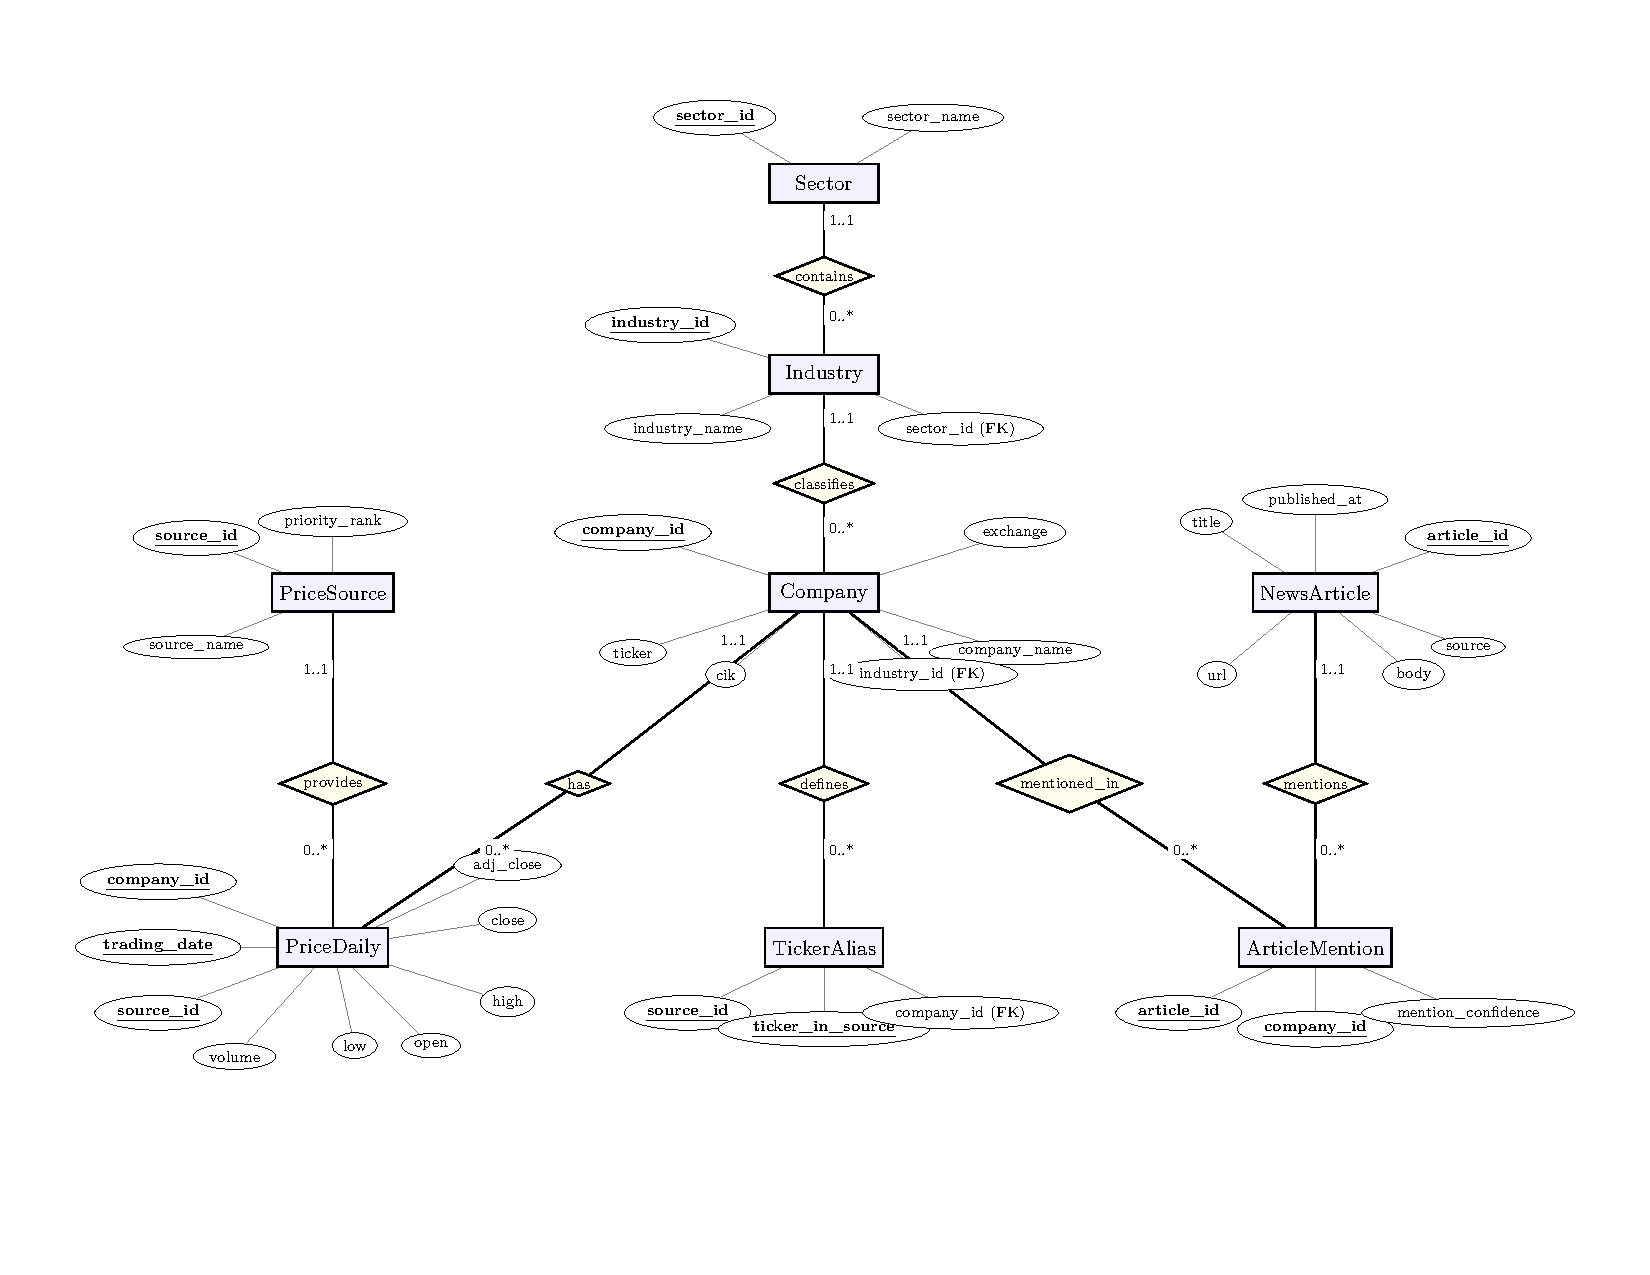
\includegraphics[width=\textwidth]{er_diagram_Chen_notation.pdf}
    %\caption{Chen Notation ER Diagram for Stock Trader}
\end{figure}

%═══════════════════════════════════════════════════════════
\newpage
\section{SQL DDL --- Creating the Database}
%═══════════════════════════════════════════════════════════

(DDL kept consistent with the ERD; includes provenance for multiple sources and a ticker-alias table for entity resolution.)

\begin{lstlisting}[style=sql,basicstyle=\ttfamily\scriptsize,aboveskip=0.5em,belowskip=0.5em]
CREATE TABLE sector (
    sector_id    SERIAL PRIMARY KEY,
    sector_name  TEXT NOT NULL UNIQUE
);
CREATE TABLE industry (
    industry_id    SERIAL PRIMARY KEY,
    industry_name  TEXT NOT NULL,
    sector_id      INT NOT NULL REFERENCES sector(sector_id),
    UNIQUE (sector_id, industry_name)
);
CREATE TABLE company (
    company_id    SERIAL PRIMARY KEY,
    ticker        TEXT NOT NULL UNIQUE,
    company_name  TEXT,
    exchange      TEXT,
    cik           TEXT,
    industry_id   INT REFERENCES industry(industry_id)
);
\end{lstlisting}

\newpage

\begin{lstlisting}[style=sql]
CREATE TABLE price_source (
    source_id      SERIAL PRIMARY KEY,
    source_name    TEXT NOT NULL UNIQUE,
    priority_rank  INT NOT NULL
);

CREATE TABLE price_daily (
    company_id    INT NOT NULL REFERENCES company(company_id),
    trading_date  DATE NOT NULL,
    source_id     INT NOT NULL REFERENCES price_source(source_id),
    open          DOUBLE PRECISION,
    high          DOUBLE PRECISION,
    low           DOUBLE PRECISION,
    close         DOUBLE PRECISION,
    adj_close     DOUBLE PRECISION,
    volume        BIGINT,
    PRIMARY KEY (company_id, trading_date, source_id)
);

-- Entity resolution: map dataset-specific tickers to canonical company_id
CREATE TABLE ticker_alias (
    source_id         INT NOT NULL REFERENCES price_source(source_id),
    ticker_in_source  TEXT NOT NULL,
    company_id        INT NOT NULL REFERENCES company(company_id),
    PRIMARY KEY (source_id, ticker_in_source)
);

-- News
CREATE TABLE news_article (
    article_id    BIGSERIAL PRIMARY KEY,
    source        TEXT,
    published_at  TIMESTAMPTZ NOT NULL,
    title         TEXT NOT NULL,
    url           TEXT UNIQUE,
    body          TEXT
);

CREATE TABLE article_mention (
    article_id            BIGINT NOT NULL REFERENCES news_article(article_id)
                          ON DELETE CASCADE,
    company_id            INT NOT NULL REFERENCES company(company_id)
                          ON DELETE CASCADE,
    mention_confidence    DOUBLE PRECISION,
    PRIMARY KEY (article_id, company_id)
);

-- Indexes for expected workloads
CREATE INDEX idx_company_industry  ON company(industry_id);
CREATE INDEX idx_price_daily_date  ON price_daily(trading_date);
CREATE INDEX idx_news_published_at ON news_article(published_at);
CREATE INDEX idx_mention_company   ON article_mention(company_id);
\end{lstlisting}

%═══════════════════════════════════════════════════════════
\section{Cleaning and Preprocessing Plan}
%═══════════════════════════════════════════════════════════

We will standardize identifiers, normalize schemas across sources, and deduplicate carefully to support efficient queries and later entity resolution.

\subsection{A) Canonical identifiers + entity resolution}

\begin{itemize}
    \item Create canonical company(company\_id, ticker, \ldots) keyed by company\_id.
    \item Normalize tickers (uppercase, trim, unify punctuation).
    \item Populate ticker\_alias(source\_id, ticker\_in\_source $\rightarrow$ company\_id) for source-specific quirks.
\end{itemize}

\subsection{B) Multi-source price ingestion}

\begin{itemize}
    \item For each Kaggle price dataset (e.g., ``Stock Market Data'' and ``U.S.\ Stock Dataset''), load into staging, then normalize into price\_daily.
    \item Use price\_source.priority\_rank to define a ``preferred'' source when duplicates exist.
    \item De-dup logic: if multiple sources provide the same (ticker, date), keep all rows (for provenance).
\end{itemize}

\subsection{C) Sector + industry classification}

\begin{itemize}
    \item Even if your price datasets include labels, we will still maintain explicit sector and industry dimension tables for cleanliness and join performance.
    \item If classification differs across sources, choose a canonical mapping dataset (small) or define reconciliation rules (priority source, majority vote, etc.).
\end{itemize}

\subsection{D) News ingestion}

\begin{itemize}
    \item Choose a ticker-tagged Kaggle news dataset (recommended: ``Daily Financial News for 6000+ Stocks'' or ``News Headlines + Tickers'') and ingest:
    \begin{itemize}
        \item article fields $\rightarrow$ news\_article
        \item (article, ticker) links $\rightarrow$ article\_mention
    \end{itemize}
    \item If the dataset already provides tickers, article\_mention is straightforward; if it provides company names, we map to tickers via canonical company table.
\end{itemize}

%═══════════════════════════════════════════════════════════
\newpage
\section{Web Application Tech Tools}
%═══════════════════════════════════════════════════════════

We will build a three-tier client--server web app following the course's web architecture framing: React in the browser, Node/Express on the server, and PostgreSQL as the database.

\subsection{Database / Hosting}
\begin{itemize}
    \item \textbf{PostgreSQL} hosted on \textbf{AWS RDS} (Milestone 3+). The server connects via the \texttt{pg} npm driver using the RDS endpoint on port 5432, with credentials stored in environment variables.
    \item Following the course's \textbf{Embedded SQL} approach, we write parameterized SQL directly in application code (no ORM), giving full control over joins, window functions, and aggregations.
\end{itemize}

\subsection{Backend}
\begin{itemize}
    \item \textbf{Node.js + Express} for the API layer. Routes follow the \texttt{app.METHOD(PATH, HANDLER)} pattern; each handler builds a parameterized SQL query, executes it via \texttt{pool.query()}, and returns results with \texttt{res.json()}.
    \item Routes are organized into \texttt{express.Router()} modules: \texttt{/api/companies}, \texttt{/api/prices}, \texttt{/api/sectors}, \texttt{/api/compare}, and \texttt{/api/news}.
    \item Core dependencies: \texttt{express}, \texttt{pg}, \texttt{dotenv} (env-var loading), \texttt{cors} (cross-origin requests between React dev server and Express).
\end{itemize}

\subsection{Frontend}
\begin{itemize}
    \item \textbf{React.js} scaffolded with \texttt{create-react-app}. All components are functional, using \texttt{useState} for local state and \texttt{useEffect} to trigger \texttt{fetch()} calls to the Express API on load or filter changes.
    \item \textbf{React Router} provides client-side routing across the four main pages (Home, Sector/Industry, Compare, News Explorer) without full page reloads.
\end{itemize}

\subsection{Updates / Transactions}
\begin{itemize}
    \item For multi-step writes (e.g., watchlist updates), we wrap sequences in explicit transactions (\texttt{BEGIN \ldots{} COMMIT/ROLLBACK}). Default isolation is \textbf{READ COMMITTED}; we will only strengthen it if a specific feature requires it.
\end{itemize}

%═══════════════════════════════════════════════════════════
\newpage
\section{Team Responsibilities}
%═══════════════════════════════════════════════════════════

Because we are currently a 3-person team, we will have to distribute more work per person and have each person take more responsibility for a subsection of the web application.

\begin{enumerate}[label=\textbf{\arabic*.}]
    \item \textbf{Philip Lee (ETL, entity resolution and normalization):}\\
    Organize and normalize into price\_daily; create/maintain canonical company, industry, sector, and ticker\_alias; document cleaning rules.

    \item \textbf{Na Ni (DB + SQL lead):}\\
    Finalize ERD + DDL; implement complex SQL queries (leaderboards, anomalies, correlation helpers); indexing strategy; performance testing plan.

    \item \textbf{Kartheek Gavini (Full-stack app lead):}\\
    Design and implement Express API endpoints (route structure, parameterization, error handling); build React page components and data-fetching logic; wire the end-to-end pipeline from browser to database; integration testing; deployment wiring (local + AWS later).
\end{enumerate}

\end{document}